\chapter{Algorithm Analysis}

\section{Traffic Analysis}



A SDN based IoT infrastructure basically provides free-flow of data from sensors and wireless devices and the efficiency of the network depends on the management and security of traffic. Network traffics are dynamic and hence its more prone to malicious attacks such as DDOS, MITM, Replay, Side Channel etc.

\subsection{Traffic Analysis Technique}

There are various classification techniques to classify the network traffic, but among these the following three techniques are mostly used-port based, payload/DPI (Deep Packet Inspection) based and ML (Machine Learning)-technique.

In \textbf{Port-based technique}, IP addresses are identified and used to classify the corresponding applications which are registered under Assigned Number Authority (AINA). In the other side, \textbf{Payload-based} or \textbf{Deep Packet Inspection(DPI)} are basically used to classify dynamic port numbers (peer to peer applications) and packets are analyzed for signatures and authentications of network applications of traffic.\textbf{ ML (Machine Learning)-technique} uses trained classifiers as input for traffic classification based on the data set.

For our proposed system, to analysis the traffic efficiently we are applying ML-technique, as port-based classification doesn’t provide the identification of dynamic ports and payload-based doesn’t work for encrypted traffic and requires continuous updating of signature patterns of new applications. ML-technique overcomes these shortcomings of the following classification techniques and works more efficiently to classify data packets \cite{6091325,Santi-journal}.


\begin{figure}[ht]
    \centering
    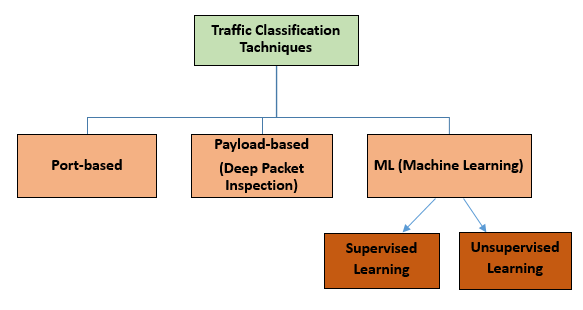
\includegraphics{Chap4/trafficanalysis.png}
    \caption{Traffic Analysis Technique}
    \label{fig:traffic_analysis}
\end{figure}

\textbf{ML (Machine Learning)- Technique}

Machine learning is used for dynamic analysis for traffic and uses \textbf{WEKA} tool for detection method. It has two techniques for classification- supervised and unsupervised. In \textbf{Supervised} technique there is a training data set as input to train the system model for the expected output but in \textbf{unsupervised} technique there is no training/known data set and it works based on the prior knowledge or the statistical information.



\section{Feature Extraction}

By analyzing the network traffic, we get a data set which is the combination of the malware and benign data packets and this is the first major component for any malware detection system. A feature extractor is used to extract the features from the specified data set and we need to extract a group of features to detect attacks, which is not possible by extracting any specific or single feature.

\subsection{Feature Extraction Tool}
Here we are using the \textbf{Wireshark} and \textbf{Net Mate tool} for the corresponding live data packet capturing and feature extraction purpose.
\begin{enumerate}
    \item \textbf{Wireshark:} Wireshark is an open source software and an efficient network packet analyzer. Wireshark captures the network traffic from various wireless devices and displays them with very detailed protocol information and save the captured data packet. It can also export some or all packets in a number of capture file formats and filter them on many criteria. The basic features of Wireshark tools are-
    \begin{itemize}
        \item Capture traffics from live network or read data from already captured file.
        \item Terminal version, named Tshark or GUI is used to browse captured traffic.
        \item Display filter is used to refine and edit traffic programmatically.
        \item For dissecting protocols, Plug-ins is developed.
        \item Captured traffic can be used to detect VoIP calls when compatible encoding is used for encoding. 
        \item Only selected traffic appears with several timers, settings and filters.
    \end{itemize}
    \item \textbf{Net Mate Tool:} After capturing data packets, the features are extracted using Net Mate tool as features depict the behavioral description of traffic. Net Mate includes two types of modules:
    \begin{itemize}
        \item Packet Processing Modules designed to implement different metrics 
        \item Export Module that implement different output module
    \end{itemize}
    Our concerned flow features are implemented in \textbf{Packet Processing Module}. Two different types of rules are used to produce the output: description rules and recognition rules.
\end{enumerate}
\begin{figure}[ht]
    \centering
    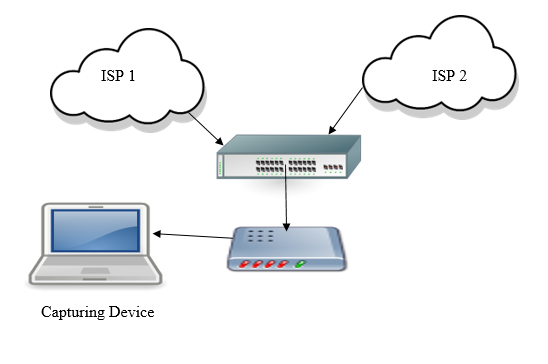
\includegraphics[width=5in]{Chap4/FeatureExtraction.PNG}
    \caption{Feature Extraction Process}
    \label{fig:feature_extraction}
\end{figure}
\section{Feature Selection}

Feature Selection is an important step after traffic analysis to detect the abnormality occurring in a system. It can be defined as automatic selection of attributes in data samples that are most relevant to the predictive modeling problem. It does the mapping to excludes the irrelevant or redundant attributes and specifically defines most prominent for the better performance of the system.

As in our proposed system we are working on a large amount of a traffic of a network so feature selection should be done for the following requirements:
\begin{itemize}
    \item To create an accurate predictive model that will give a better accuracy whilst requiring less data.
    \item it reduces the complexity of a model and makes it easier to interpret the required result.
    \item It enables the model to train faster on data sample as there is no redundant attributes.
    \item This method also reduces the problem of over fitting by enhancing the generalization in the model.
\end{itemize}
\subsection{Selection Method}
There are mainly three methods that are used in feature selection:
\begin{enumerate}
    \item \textbf{Filter Method:} Here features are selected on the basis of their scores in various statistical tests for their correlation with the outcome variable which is Machine Language Independent.\textbf{Pearson’s Correlation, LDA, ANOVA, Chi- Square}  are the methods which are used to define correlation among the features.
    \item \textbf{Wrapper Method:} This method considers the selection of a set of features as a search problem or algorithm to validate the prediction where different combinations are prepared, evaluated and compared to other combinations. After evaluating it assigns a score based on model accuracy. It can always provide the best subset of features. But this method has a high computational cost.
    \item \textbf{Embedded Method:} This method tries to combine the efficiency of other two methods and performs the selection of variables in the process of training and is usually specific to given learning machines. It basically learns which features best contribute to the accuracy of the model while the model is being created. Most common algorithms are the \textbf{LASSO, Elastic Net, Ridge Regression}used in this method.
\end{enumerate}

For our model \textbf{Wrapper Method} is most applicable. As at first we have analyzed network traffic and after that we have implemented a Search process for extracting Unusual features to detect our attacks. From the complete list of Feature set we have further selected the most effective features to make our feature domain more powerful.

\subsection{Selection Tool}
The immediate step after feature extraction of any attack detection procedure is feature selection which is the final input feature set to feed into the system by using any machine learning technique. To select the desired features from the extracted features set, an efficient tool-set, WEKA is used in our attack detection process.

\textbf{WEKA:} WEKA, (Waikato Environment for Knowledge Analysis), named after a flightless New Zealand bird, supports many feature selection techniques, i.e. correlation based, information gain based, learner based etc. Weka is a set of machine learning algorithms for data mining tasks. The algorithms can be used directly on dataset or it can be called from Java code. 

Weka contains tools for data pre-processing, classification, regression, clustering, association rules, and visualization. It provides SQL access with assistance of Java Database Connectivity. Weka provides four UI:
\begin{itemize}
    \item Explorer
    \item Experimenter
    \item KnowledgeFlow
    \item Simple CLI.
\end{itemize}
Explorer is the main user interface of Weka which have following panels:
\begin{enumerate}
    \item \textbf{Preprocess:} Choosing the data file.
	\item \textbf{Classify:} Applying and experimenting with different algorithms on preprocessed data files.
	\item \textbf{Cluster:} Applying different clustering tools, which identify clusters within the data file.
	\item \textbf{Association:} Applying association rules, which identify the association within the data.
	\item \textbf{Select attributes:} Seeing the changes on the inclusion and exclusion of attributes from the experiment.
	\item \textbf{Visualize:} Seeing the possible visualization produced on the data set in a 2D format, in scatter plot and bar graph output.
\end{enumerate}
The user cannot move between the different tabs until the initial preprocessing of the data set has been completed. This procedure can also be done with component based KnowledgeFlow and from Simple CLI. Experimenter provides option to compare predictive performance of machine learning algorithms on data-sets. 

\section{Feature Specification on Proposed Model}

From extraction procedure eighteen features are collected which are grouped into nine features for the convenience of our work.And these nine features are taken as input for the further process.The mapping or selection of features are simplified as the below figure \ref{fig:feature}
\begin{figure}[ht]
    \centering
    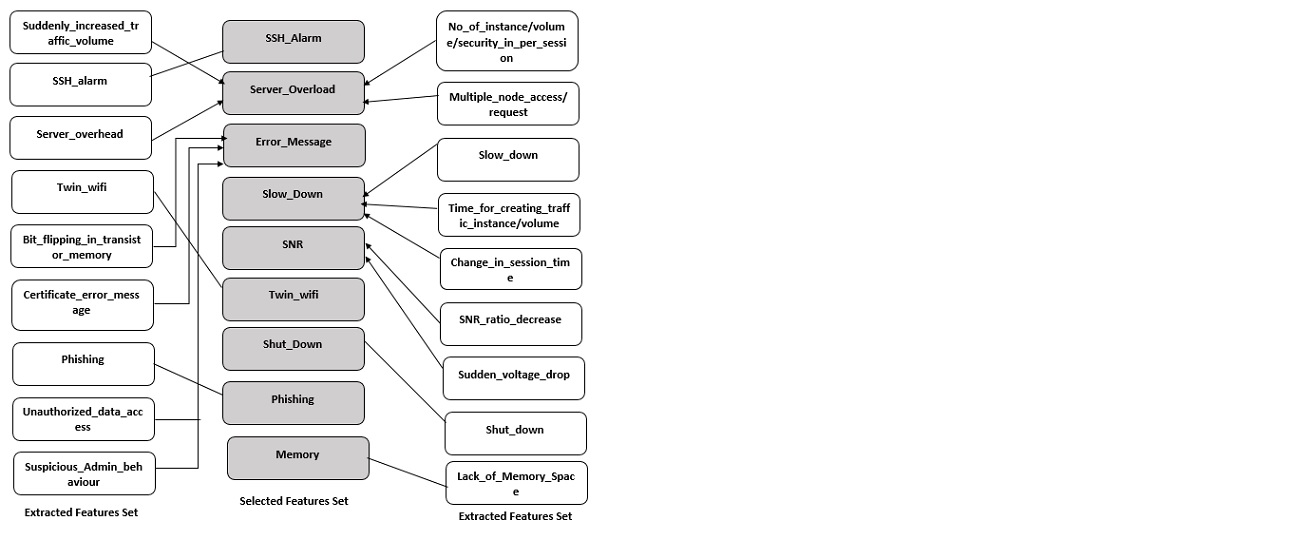
\includegraphics{Chap4/feature.jpg}
    \caption{Feature Extraction and Selection}
    \label{fig:feature}
\end{figure}

\begin{enumerate}
 \item \textbf{Server Overload:} It is one of the most common feature that happens in any kind of physical layer attack in the network. Increase of volume of data packets, excessive traffic is the indication of Server Overload. Though it’s a common feature but there is possibility of Side Channel Attack, Malicious Code and DDoS attack. 
\item \textbf{Slow Down:} It’s a common feature of DDoS and Malicious Code Attack. In DDoS there creates traffic floods in bandwidth and resources so the performance evaluation becomes very poor. It is definitely a symptom that something is wrong with the system. In malicious code there occurs illegitimate actions which creates load on the system.


\item \textbf{Sudden shut Down:} It’s the extreme case of DDoS attack in the network. a denial-of-service attack (DDoS attack) is a cyber-attack in which the perpetrator seeks to make a machine or network resource unavailable to its legitimate users by temporarily or indefinitely disrupting services of a host connected to the internet. So when network will not able to manage the overload it will just shut down.
\item \textbf{Error Message:} It is the most common characteristics of attacks that frequently occurs in IoT network model. It will generate automatically from the Operating System when it will suspect unusual activities in the network. So it is a great source of predicting that there is a third party in the network who is trying to do something illegal in the network. Features-Bit flipping in memory cells, Suspicious Admin Behavior, Unauthorized Data Access are redundant which is mapped to exclude after feature selection method. Because all these three activities are unusual and it will result an error message. DDoS, Side Channel Attack, Malicious Code Attack, Man in The Middle(MITM) attack can be suspected by this feature.
\item \textbf{	SSH Alarm:} SSH is one of the most popular communication protocols on the Internet used by admins, developers. SSH alarm is an email alert, when someone logs server via SSH (Server Secure Shell) can be pretty useful to track who is actually using server. It’s a very unique feature to track MITM attack as an intruder might not login at first attempt.
\item \textbf{Twin-WiFi:} In MITM the main aim of an intruder is to entry the network and hampers the integrity, confidentiality, authenticity of admin. To get illegal access he can adapts the method of duplicate WiFi SSID or Address that is a very prominent feature to identify that the system is being attacked by the third party.
\item \textbf{Phishing:} It’s a great threat to the security of users. It is actually a cybercrime in which targets are contacted by email, telephone or text message by someone posing as a legitimate institution to lure individuals into providing sensitive data such as personally identifiable information, banking information, credit card details, and passwords. Intruder who conducts MITM attack mostly does this to earn in an illegal way.
\item \textbf{SNR decrease:} When noise of a system increases the SNR decreases that indicates the poor performance of the system. Voltage drops with proportional to SNR, that is not definitely a good symptom for a model. It is the most prominent feature to detect the Side Channel Attack. it is caused by the information gained from the network so the noise increases which should be noticed to detect attack.
\item \textbf{Lack of Memory Space: }Malicious code is an application security threat that cannot be efficiently controlled by conventional antivirus software easily. It describes a broad category of system security terms that includes attack scripts, viruses, worms, Trojan horses, backdoors and malicious active content. So sometimes it suddenly just occupies the memory space of user device and gives warning to the user of “Memory is Full”. That’s definitely occurs a great problem of storing.

Here FIS will primarily work on these \textbf{Nine} Selected features where rules will be considered in controller to identify DDoS, MITM, Malicious Code Attack and Side Channel Attack. Rules are defined according to the priority of the features.
\end{enumerate}


